\documentclass[12pt]{article}
\usepackage{amsmath}
\usepackage{amssymb}
\usepackage{amsthm}
\usepackage{cite}
\usepackage[margin=1.35in]{geometry}
\usepackage{graphicx}
\usepackage{hyperref}
\usepackage{mathtools}
\usepackage{multirow}
\usepackage{tabularx}
\usepackage{thmtools}
\usepackage{wrapfig}

\title{Sigma Network}
\author{Daniel Lubarov\\daniel@lubarov.com}
\date{DRAFT Version 0.1\\\today}

\setlength{\intextsep}{0pt}

% Theorem definitions.
\declaretheorem{theorem}
\declaretheorem{lemma}

% We want autorefs to say e.g. "section 8.1" rather than "subsection 8.1".
\let\subsectionautorefname\sectionautorefname
\let\subsubsectionautorefname\sectionautorefname

% Integer interval notation; from https://tex.stackexchange.com/a/304670/99124
\newcommand{\isep}{\mathrel{{.}\,{.}}\nobreak}

% \floor{...}, \ceil{...}, \angled{...}.
\DeclarePairedDelimiter{\floor}{\lfloor}{\rfloor}
\DeclarePairedDelimiter{\ceil}{\lceil}{\rceil}
\DeclarePairedDelimiter{\angled}{\langle}{\rangle}

\begin{document}
\maketitle

\begin{abstract}
  We introduce Sigma Network, a cryptocurrency protocol which provides strong privacy guarantees using zero knowledge proofs. In contrast to existing privacy-oriented protocols, our blockchain design is based on proof of stake, which opens the door to a number of improvements.

  We introduce a novel, leaderless BFT consensus algorithm to quickly finalize each block, thereby eliminating forks. Under normal conditions, our algorithm achieves consensus after just two rounds of one-way communication. We prove the algorithm's safety under a 2/3 honest majority assumption, and prove its liveness under a partial synchrony assumption.

  Our protocol is designed with the expectation that each validator node will be run by multiple servers. We divide blocks into small shards, and our peer discovery protocol matches peers with overlapping shard ranges. This allows transaction volume to scale without any practical limits.

  To support users who lack the resources to process all transactions, we propose a unique light client model. Instead of verifying all transactions in a block, light clients verify that BFT consensus was achieved. Under our honest majority assumption, light clients enjoy the same security as full validator nodes, and since vote counts are not affected by transaction volume, this model allows the network to scale without increasing computational requirements for ordinary users.

  While existing cryptocurrencies have generated a great deal of interest and investment, fiat currencies remain ubiquitous in day-to-day life. Sigma Network's unique combination of privacy, scalability and low latency make it a strong candidate for adoption in everyday commerce.
\end{abstract}

\newpage
\tableofcontents
\newpage

\section{Background}
\label{background}

The success of Bitcoin demonstrates a strong interest in decentralized currencies, where monetary policies are determined by a community of users rather than government decree. Bitcoin's purported anonymity contributed to its success, but a growing body of research shows that accounts can often be deanonymized based on their public activity \cite{meiklejohn2013fistful} \cite{androulaki2013evaluating}.

Some newer cryptocurrencies improve upon Bitcoin's privacy. Monero \cite{van2013cryptonote} uses ring signatures to obfuscate a transaction's source of funds, and Diffie-Hellman exchanges to hide its destination. Similarly, Zcash \cite{sasson2014zerocash} uses zk-SNARKs to prove that a transaction has a valid source of funds without revealing what that source is. Zcash's privacy guarantee is stronger by comparison, since its shielded transactions leak no information at all, whereas Monero uses rings of size 7 by default.

While Zcash and Monero offer strong privacy, both protocols are designed to be executed by individual computers, so their transaction volume is limited by the capabilities of a single machine. Both protocols have sufficient capacity for the current transaction volume, but their limited scalability precludes their adoption in mainstream commerce.

Another drawback of Bitcoin, Zcash and Monero is that they rely on proof of work for consensus. The security model fundamentally requires that mining be expensive, as this creates an economic barrier to 51\% attacks. At the time of writing, Bitcoin mining is funded by about \$4 billion worth of block rewards per year, which causes an inflation rate of about 4\%.% As the block reward decreases, inflation will decrease, but transaction fees will need to increase in order to maintain the same security level. In one way or another, Bitcoin users must fund mining operations in order to maintain adequate security.

Yet another challenge is latency. Bitcoin has an average block time of 10 minutes, and \cite{nakamoto2008bitcoin} recommends waiting for six confirmations before accepting a transaction as final. Some newer cryptocurrencies such as Tendermint \cite{kwon2014tendermint} and Algorand \cite{chen2018algorand} provide quick finality using BFT consensus algorithms, but they are subject to the same privacy issues as Bitcoin.

Finally, most existing cryptocurrencies do not offer post-quantum security. This includes Zcash and Monero, both of which rely on the hardness of the discrete logarithm problem for transaction soundness. A universal quantum computer could compute discrete logarithms in polynomial time using a variant of Shor's algorithm. To date, Shor's algorithm has been demonstrated only with very small factorization problems \cite{martin2012experimental}. Still, the potential future impact of quantum computers is a cause for concern.

Our design aims to address all of the aforementioned challenges. It offers a strong privacy guarantee using zero knowledge proofs, similar to Zcash, but using a post-quantum secure proof system based on multiparty computation. Our blockchain protocol is based on proof of stake, so security is inexpensive compared to proof of work blockchains. We use use a novel BFT consensus algorithm to quickly finalize each block, thereby ensuring immutability and eliminating forks. To allow transaction volume to scale, we use a simple sharding mechanism which lets each validator divide their communications among multiple servers.

\section{Protocol overview}
\label{protocol}

Sigma Network organizes protocol state into a blockchain structure. We use a BFT algorithm, described in \autoref{consensus}, to commit a single (possibly empty) block at each height. Because exactly one block is committed at each height, committed blocks form a path. And because all valid blocks at the same height must share the same committed parent, valid blocks form a caterpillar tree.

\begin{figure}[h]
  \centering
    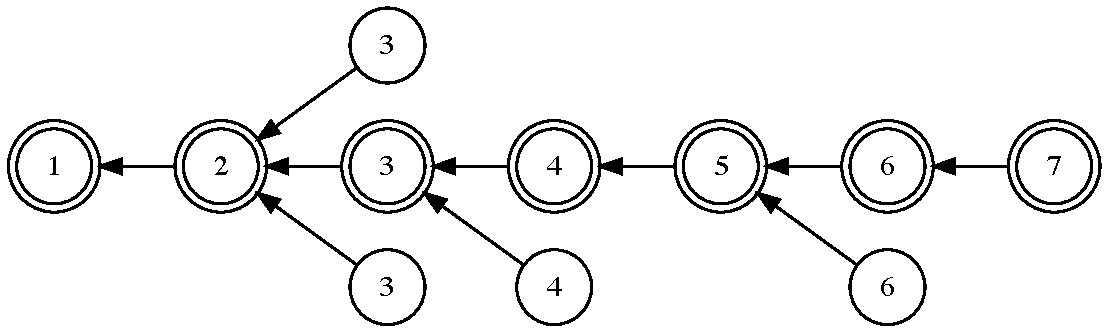
\includegraphics[width=0.7\textwidth]{images/chain-structure}
  \caption{A possible composition of valid blocks. The numbers represent block heights, and the double circles represent committed blocks.}
\end{figure}

This structure has several benefits. Since blocks are committed shortly after they have propagated, transactions are confirmed very quickly, with a strong guarantee of irreversibility. Additionally, blocks can be generated as quickly as the network is able to propagate them; the BFT process eliminates the need for fixed block timing. Finally, the lack of forks makes client performance very predictable.

% TODO: Explicitly define validators.

A validator must register as a block creator before being eligible to create a block, and must register as a voter before being eligible to vote in the BFT consensus protocol. These registration messages are similar to transactions---they must be included in a block before they are recognized, and they may include transaction fees in order to incentivize inclusion.

Each registration message has an associated score, which is pseudorandomly generated based on some account data. An account must have a certain minimum amount of stake, \texttt{DepositAmount}, in order to submit any registrations. The more stake an account has, the more registrations they may submit, each with a unique score.

If more than one validator registers to create the same block, only the one with the highest score is eligible to do so. Similarly, if more than \texttt{MaxVoters} register to vote in the same epoch, only the highest-scoring \texttt{MaxVoters} are eligible to do so.

Blocks are grouped into \emph{epochs}, each consisting of \texttt{EpochSize} blocks. If a validator wishes to participate in epoch $i$, they must submit their registration during epoch $i - 1$. Since there are many blocks in an epoch, validators have many opportunities to have their registration messages included. Censoring registration messages would be difficult, since it only takes a single uncooperating block creator to thwart a censorship attempt by including any pending registrations.

\section{Validator registration}
\label{registration}

% TODO: mention ability to submit registration messages from another account, to pay fees without invalidating the main account
% registrations included in block headers
% separate registrations limit for light clients

In each epoch, validators may register to create blocks or vote in the following epoch. Since the process is similar for both, we describe a generic protocol for event registration.

A validator may register for an event by submitting one or more \emph{tickets}. A validator with a stake of $s$ may submit up to $\floor{s / \mathtt{DepositAmount}}$ tickets per event, each with a unique index $i$.

Each ticket has a score, which is computed as
\[ R(x, \mathrm{sk}, e, i) \]
where $R$ is a pseudorandom function, $x$ is the random seed of the current epoch, $\mathrm{sk}$ is the validator's secret key, $e$ is an event identifier, and $i$ is the ticket index.

A registration message includes a non-interactive zero-knowledge proof (NIZKP) showing that a certain ticket was scored correctly. The event $e$ is a public input to the NIZKP, but $\mathrm{sk}$ and $i$ are private, so no account data is revealed. The details of the NIZKP circuit are covered in \autoref{registration-circuit}.

At the end of an epoch, tickets are approved or denied based on their ranking. For block creation events, only one ticket is approved at each block height. For voting events, the top \texttt{MaxVoters} tickets are approved to vote in the next epoch.

Since ticket scores are public, validators can often judge whether their ticket is likely to be approved based on the scores of any previously submitted tickets. Validators can save on transaction fees by not submitting tickets which are likely to be denied.

\section{Entropy collection}
\label{entropy}

When a validator creates a new account, it is important that they not be able to predict its ticket scores. Otherwise, a validator could enumerate possible key pairs until they eventually find one with high-scoring tickets. To prevent such ``grinding'' attacks, we use a new random seed in each epoch. A validator account created in epoch $i$ cannot submit tickets until epoch $i + 2$, so there is a full round of entropy generation in epoch $i + 1$ before the account becomes eligible.

The random seed for each epoch is derived from the signatures of block creators. In particular, each block creator submits $\operatorname{R}(\mathrm{sk}, h)$ as their entropy contribution, where $R$ is a pseudorandom function, sk is their secret key and $h$ is the height of the block. This is one of the outputs of the NIZKP given by each block creator, which is described in \autoref{block-creation-circuit}.

At the end of each epoch, these entropy submissions are xor'd together, and the resulting number becomes the random seed of the following epoch.

Since this computation is deterministic, the only way for a validator to influence entropy is to skip their block. Consider the validator $\nu$ who is eligible to create the last $n$ blocks in some epoch $i$. (Typically $n = 1$, but $\nu$ could get lucky and have several contiguous blocks at the end of the epoch.) $\nu$ may manipulate $n$ bits of entropy by creating or withholding blocks. In other words, $\nu$ can choose from $2^n$ random seeds for epoch $i + 1$. If they do withhold blocks, they will miss out on the block reward, but it may occasionally be profitable if it results in a more favorable random seed for the next epoch.

[TODO: Need some analysis to show that manipulation is rarely profitable, and that there's negligible effect on the equitable distribution of block rewards.]

[RANDAO is reasonable alternative---we can slash validators who withhold their entropy contribution rather just relying on the block reward as a minor incentive. However, I think the analysis will show that it's unnecessary; profitable manipulation will be rare either way.]

[Also considering verifiable delay functions which can provide manipulation-proof entropy, but it may be best to wait for new developments in this very new field. \cite{wesolowski2018slow} seems practical, but relies on discrete log hardness.]

\section{BFT consensus algorithm}
\label{consensus}

\newcommand{\vote}[1]{\angled{#1}}
\newcommand{\preparevote}[1]{\vote{\mathtt{PREPARE}, #1}}
\newcommand{\commitvote}[1]{\vote{\mathtt{COMMIT}, #1}}
\newcommand{\prepared}[2][]{\operatorname{prepared}_{#1}(#2)}
\newcommand{\committed}[2][]{\operatorname{committed}_{#1}(#2)}

In everyday commerce, transaction latency is of paramount importance. While some users may be willing to accept transactions without a guarantee of finality, others require such a guarantee in order to eliminate counterparty risk. For this reason, we use a Byzantine fault tolerant consensus algorithm to finalize each block as soon as it has been propagated through the network.

Note that our algorithm is special purpose; we leverage certain properties of our blockchain design in order to guarantee convergence without relying on leaders. The algorithm would not work with arbitrary values; such a generalization would invalidate our proof of liveness.

We assume that over $2/3$ of validators are honest, meaning that they vote as prescribed below. In particular, given a set of $3t + 1$ validators, we assume that at least $2t + 1$ of them are honest, while at most $t$ are not.

We further assume that the same $2t + 1$ validators are connected with partial synchrony. Given some bounded delay $\Delta$, we assume that the system will alternate between periods of synchrony, where all messages are propagated among this $2t + 1$ validator set, and periods of asynchrony, where messages are lost or delayed beyond $\Delta$.

Voting takes place over a series of rounds. For the moment, we will assume that some rounds are wholly synchronous, meaning that all votes are propagated among this $2t + 1$ validator set before any of them consider the round to have terminated. Because of timing issues, this does not immediately follow from our partial network synchrony assumption, but we will justify this stronger assumption in \autoref{round-timing}.


\subsection{Definitions}

We define two types of votes. $\preparevote{\nu, b, r}$ signifies that some validator $\nu$ votes to prepare block $b$ in round $r$. $\commitvote{\nu, b, r}$ signifies that $\nu$ votes to commit $b$ in round $r$. Both messages are accompanied by signatures to ensure authenticity. Note that validators may vote for an empty block; we denote this with $b = \emptyset$.

Next, we define the predicate $\prepared{b, r}$ to be true if and only if $b$ has received at least $2t + 1$ votes of either kind in round $r$. We define $\committed{b, r}$ to be true if and only if $b$ has received at least $2t + 1$ \texttt{COMMIT} votes in round $r$.

Further, we define $\prepared[\nu]{b, r}$ to be true if and only if $\nu$ knows $\prepared{b, r}$ to be true based on the votes that $\nu$ has observed. Similarly, we define $\committed[\nu]{b, r}$ to be true if and only if $\nu$ knows $\committed{b, r}$ to be true.


\subsection{Voting rules}

In each round $r$, each honest validator $\nu$ votes as follows.
\begin{enumerate}
  \item If $\prepared[\nu]{a, s}$ for some block $a$ and round number $s$, then let $s, a$ be the highest such round number and the associated block.
    \begin{enumerate}
      \item If $s = r - 1$, then $\nu$ votes $\commitvote{\nu, a, r}$.
      \item Otherwise, $\nu$ votes $\preparevote{\nu, a, r}$.
    \end{enumerate}
  \item Otherwise, let $B$ be the set of valid blocks that $\nu$ has received for this block height.
    \begin{enumerate}
      \item If $B$ is a singleton set $\{ b \}$, then $\nu$ votes $\preparevote{\nu, b, r}$.
      \item Otherwise, $\nu$ votes $\preparevote{\nu, \emptyset, r}$.
    \end{enumerate}
\end{enumerate}
Each validator $\nu$ halts as soon as $\committed[\nu]{b, r}$ for any $b, r$. $\nu$ will then accept $b$ as the final, irreversible block for the current block height.


\subsection{Proving safety and liveness}

\begin{lemma}\label{also-prepared}
  \( \committed{b, r} \) implies \( \prepared{b, r} \).
\end{lemma}

\begin{proof}
  This follows immediately from our definitions. $\committed{b, r}$ entails that $b$ received at least $2t + 1$ \texttt{COMMIT} votes. This also satisfies the definition of $\prepared{b, r}$, which counts votes of either kind.
\end{proof}

\begin{lemma}\label{uniqueness}
  At most one block will become prepared at each round number.
\end{lemma}

\begin{proof}
  Assume the opposite: $\exists a, b, r$ such that $\prepared{a, r}$ and $\prepared{b, r}$. Then both $a$ and $b$ received $2t + 1$ or more votes in round $r$, for a total of $4t + 2$ or more votes. Since there are only $3t + 1$ validators, at least $t + 1$ of them must have voted for both $a$ and $b$, which violates our assumption that at most $t$ validators are dishonest.
\end{proof}

\begin{lemma}\label{finality}
  $\nexists a, b, r, s$ such that $\committed{a, r}$, $\prepared{b, s}$, and $s > r$.

  Equivalently, if some block is committed, no block may be prepared in a later round.
\end{lemma}

\begin{proof}
  Suppose $\committed{a, r}$. Then by definition, $2t + 1$ validators must have voted $\commitvote{\nu, a, r}$, and by our honesty assumption, at least $t + 1$ of these votes must have come from honest validators. For each of these validators $\nu$, we know $\prepared[\nu]{a, r - 1}$, otherwise $\nu$ would not have followed rule 1a.

  By the logic of rule 1, these $t + 1$ honest validators will continue voting for $a$ until a different block becomes prepared. This leaves $(3t + 1) - (t + 1) = 2t$ remaining validators who may vote for a different block. Since $2t$ is one short of a quorum, a different block will never gain enough votes to become prepared.
\end{proof}

\begin{theorem}[Safety]
  At most one block will become committed.
\end{theorem}

\begin{proof}
  Assume the opposite: $\exists a, b, r, s$ such that $\committed{a, r}$ and $\committed{b, s}$. \autoref{uniqueness} implies $r \ne s$. Without loss of generality, assume $r < s$. \autoref{also-prepared} implies $\prepared{b, s}$, which contradicts \autoref{finality}.
\end{proof}

\begin{theorem}[Liveness]
  It is always possible for a block to become committed.
\end{theorem}

\begin{proof}
  Let $r$ be the current round. Let $B$ be the set of valid blocks which have propagated to at least $2t + 1$ honest validators before they begin round $r$. Consider these possible protocol states:
  \begin{enumerate}
    \item $\nexists b, s$ such that $\prepared{b, s}$, and $|B| = 0$.
    \item $\nexists b, s$ such that $\prepared{b, s}$, and $|B| = 1$.
    \item $\nexists b, s$ such that $\prepared{b, s}$, and $|B| \ge 2$.
    \item $\exists b, s$ such that $\prepared{b, s}$, but all such $s < r - 1$.
    \item $\exists b$ such that $\prepared{b, r - 1}$.
    \item $\exists b, s$ such that $\committed{b, s}$.
  \end{enumerate}
  We will show that in a synchronous round, the protocol will always progress to a state with a higher number. In an asynchronous round, it is possible for the protocol to regress from state 5 to state 4, but it will cycle between 4 and 5 until there is eventually a transition from 5 to 6.

  If the current state is 1, then validators will vote in accordance with rule 2. If a valid block has been released but not fully propagated, it will be propagated this round, advancing us to state 2. If not, all honest validators will vote to prepare $\emptyset$ as per rule 2b, advancing us to round 5.

  If the current state is 2, then the logic is similar. If two or more valid blocks have been released but only one has fully propagated, then a second block will be propagated this round, advancing us to state 3. If not, the $2/3$ of honest validators who have seen one block will vote for that block as per rule 2a, advancing us to round 5.

  If the current state is 3, then the honest $2/3$ of validators will vote for $\emptyset$ as per rule 2b, advancing us to round 5.

  If the current state is 4, then honest validators will vote $\preparevote{\nu, b, r}$ in accordance with rule 1b. Thus upon the completion of round $r$, we have $\prepared{b, r}$, which puts us in state 5 for round $r + 1$.

  If the current state is 5, then honest validators will vote $\commitvote{\nu, a, r}$ in accordance with rule 1a, resulting in a successful commit, thereby advancing us to state 6 which is terminal.
\end{proof}


\subsection{Round timing}
\label{round-timing}

In our protocol, the timing of rounds is based on when certain messages are received. Since different validators may receive the same message at different times, this introduces an element of subjectivity. However, these differences in perceived round timing are bounded by $\Delta$ during periods of synchrony.

Once a validator $\nu$ receives a valid block for some height, they consider that moment the beginning of the first round. If \texttt{BlockTimeout} elapses and $\nu$ hasn't received any valid block, they will consider the moment of the timeout to be the beginning of the first round.

Subsequently, $\nu$ considers a round $r$ to have terminated (and round $r + 1$ to have begun) when one of the following conditions have been met:

\begin{enumerate}
  \item $2 \Delta$ has elapsed since the round begun. This allows $\Delta$ for votes to propagate, and $\Delta$ to account for differences in validators' perceptions of $r$'s start time. So if the network was synchronous during this period, then all votes in round $r$ have had sufficient time to propagate.
  \item At least $t + 1$ votes have been cast in round $r + 1$. Our honesty assumption implies that at least one of these votes must be from an honest validator, so one of the other two termination conditions must have been met.
  \item $\prepared[\nu]{b, r}$ for any block $b$. In this case, \autoref{uniqueness} implies that no other block can become prepared in $r$.\footnote{It is possible that $\committed{b, r}$, and $\nu$ may not become aware of it until more votes are received. For example, if $\nu$ received one vote to prepare $b$ and $2t$ votes to commit it, they would terminate the round based on this rule. If $\nu$ later received one more vote to commit $b$, then they would learn that $b$ has been committed. In cases like this, however, there is no harm in $\nu$ terminating the round early, since the commitment would have succeeded regardless.} Note that this termination condition is not strictly necessary---we could wait for the timeout---but terminating early helps to minimize latency.
\end{enumerate}

[TODO: This part is unfinished.]


\subsection{Incentives}

Sigma Network offers neither rewards for voting nor penalties for breaking the rules. Validators already have an incentive to download vote data, since they must be prepared to create a block in the future when it is their turn. This is in contrast to protocols such as Casper FFG \cite{buterin2017casper}, which punish validators who violate a rule by slashing their funds.

The safety of our protocol relies on the difficulty of coordinating $t + 1$ validators and convincing them to participate in a joint attack. We consider this unlikely, since validators are directly invested in the success of the currency, and a successful $1/3$ attack would likely have a major impact on the value of their investment.

[TODO: Consider having validators expose their nullifiers so that, in the event of a successful $1/3$ attack, the community could coordinate a hard fork to blacklist the attacker. This seems almost as effective as Casper FFG's automatic penalties, since in in the event of a successful $1/3$ attack, an emergency hard fork would be required anyway to sort out the conflicting finalized checkpoints.]


\subsection{Related work}

Our consensus algorithm is similar to that of Tendermint \cite{kwon2014tendermint}, the main difference being that we have eliminated the propose step. In the general problem of BFT consensus, proposals play an important role in guaranteeing eventual convergence. Without proposals, voters may be split among multiple candidate values and possibly never converge, particularly if malicious voters impede convergence by voting for minority values. In the context of our blockchain design, however, the logic in rule 2 ensures convergence, as we showed in the liveness proof.

Under normal conditions, our algorithm transitions from state 1 to state 5, then to state 6. So finality is typically reached after just two rounds of communication, whereas other BFT consensus algorithms require a minimum of three rounds.

Another advantage of our leaderless voting rules is that soft forks require 67\% support, rather than 34\% support, as in proposal-based protocols like Tendermint. We discuss this further in \autoref{soft-forks}.

Our timing mechanics also differ from other BFT algorithms. While Tendermint and Algorand allocate a specific period of time for each round of voting, our protocol terminates rounds early when a block becomes prepared. This speeds up the consensus process, particularly in the common case where a single block is propagated, becomes prepared in the first round, and becomes committed in the second round.

\section{Zero knowledge proofs of validity}
\label{proofs}

We use zero knowledge proofs to demonstrate the validity of transactions, as well as other messages such as voter registration. In particular, we use the proof system described in \cite{katz2018improved}, which gives reasonable proof times and sizes for circuits with relatively small numbers of AND gates. The proof system, hash functions, and the other cryptographic primitives we use are all parameterized for 128 bit classical security.

[The proof system is subject to change. Need to evaluate zk-STARKs which purportedly were improved to ~80kb for a Zcash-like circuit? Also consider using zk-SNARKs for now, and transitioning to something else later if/when Shor's algorithm becomes more of a threat.]

The proofs described below all deal with \emph{notes}. A note is a message $\angled{\mathrm{pk}, n, s}$, where pk is the public key of the user who owns the note, $n$ is the number of coins which the note represents, and $s$ is a salt which is pseudorandomly generated by the user to sent the note.


\subsection{Spend circuit}
\label{spend-circuit}

Each transaction has one or two \emph{source} notes and zero, one or two \emph{destination} notes. The source notes are consumed by the transaction, while the destination notes are newly created. In order for a transaction to be valid, the combined amounts of the source notes must equal the combined amounts of the destination notes plus the transaction fee.

The spend circuit proves that a transaction is valid. We use a design similar to Zcash's \texttt{POUR} circuit. The circuit consumes one or two notes and produces one or two new notes. This lets users split one account into two, or combine two accounts into one, all without revealing which type of transaction they are performing.

To ensure that a note cannot be consumed twice, a ``nullifier'' associated with the note is exposed in the output layer. Validators keep track of all previous nullifiers, and reject any transactions whose nullifiers are already present in the nullifier set. An outsider cannot tell which nullifiers are associated with which commitments, but the circuit guarantees that a unique nullifier is produced for each commitment. Thus, we are able to prevent double spending without sacrificing privacy.

%\begin{figure}
%  \centering
%    \includegraphics[width=0.8\textwidth]{images/circuits/spend}
%  \caption{The structure of the spend circuit. Note that in the real circuit, there are two source notes and two destination notes, but we only depict one of each for the sake of brevity.}
%\end{figure}

Zcash stores all commitments in a Merkle tree of depth 64, using SHA-256 as the hash function. To validate that the commitments being consumed are actually present in the blockchain, the \texttt{POUR} circuit includes two Merkle proofs going all the way up to the Merkle root.

The SHA-256 circuit Zcash uses has 27,904 AND gates, and the entire \texttt{POUR} circuit has 4,109,330 AND gates.

[TODO: Explain our approach in detail. TLDR: We use LowMC-256 \cite{albrecht2015ciphers} + Davies-Meyer as the hash function. We use Merkle trees with a depth of 5, giving us an AND count of ~20k, and proof sizes well under 100kb. Our privacy guarantee is not as great as Zcash's, but better than Monero's; our default ring size is 32 compared to their default of 7. This is all tentative and subject to change.]


\subsection{Registration circuit}
\label{registration-circuit}

[TODO: Explain the circuit.]

[TODO: Add a graph to show the structure.]


\subsection{Vote circuit}
\label{vote-circuit}

[TODO: This should just be a simple signature? Preimage and message in the input layer, postimage in the output layer?]

[TODO: Add a graph to show the structure.]


\subsection{Block creation circuit}
\label{block-creation-circuit}

[TODO: This should just be a simple signature to show that a block was endorsed by the eligible block creator.]


\subsection{Performance}

[TODO: Add average case proof sizes, plus proof times and verification times.]

\section{Communication, sharding and light clients}
\label{sharding}

Most blockchain protocols were designed to be run by individual computers, which severely limits their capacity. With its current maximum block size of 1 megabyte, Bitcoin supports a theoretical maximum of 7 transactions per second. This is a far cry from global electronic payment volume; Visa's payment network, for example, has been stress tested with up to 47,000 transactions per second \cite{visa2013capacity}.

Our protocol, on the other hand, is designed to be executed by a scalable cluster of machines. At the same time, we provide a strong security guarantee for light clients, so that users can safely send and receive payments with minimal computing resources.


\subsection{Sharded block structure}

Each block $b$ is broken up into $n$ shards: $b_1, b_2, ... b_n$. Validators are free to shard transactions in any manner they choose, as long as the size of each shard does not exceed a specified maximum.

The mempool, which contains pending transactions and validator registrations, is also sharded. Regular transactions are sharded based on the nullifier of the first transaction being spent, and validator registrations are sharded based on the nullifier of the validator account. This scheme ensures that a single transaction cannot be added to multiple mempool shards, which helps mitigate mempool spam.

When a newly started node is discovering peers, it advertises the range of shards that it processes and searches for peers with overlapping ranges. Nodes should ignore any peers whose shard ranges do not overlap with their own.


\subsection{Suggested implementation strategy}

Validators are free to use any implementation strategy. They could, for example, run a full node a single server, with a high-capacity network interface and many CPUs for parallel proof verification. However, the protocol design lends itself to the following suggested implementation.

Consider a validator with $k + 1$ servers. One server is designated as the coordinator, while the $k$ remaining servers are designated as workers. The entire shard interval $[1 \isep n]$ is divided into $k$ non-overlapping intervals, and each worker is assigned one.

When the coordinator discovers a new, valid block header, it instructs each worker to download and verify the block shards assigned to it. When a worker has finished verifying a shard, it reports the validity back to the coordinator. If all shards are reported as valid, the coordinator will vote to prepare the block, as per rule 2 in the Consensus section. If one or more shards are invalid, the coordinator will vote to prepare the empty block $\emptyset$.

When a validator is eligible to create a block, each worker generates a block for each of the shards assigned to it, drawing transactions from the mempool shards assigned to them. Once a worker has finished preparing a block shard, it computes a hash of the message and reports that to the coordinator. One the coordinator has received a hash for every block shard, it broadcasts a block announcement message which contains these hashes along with other block headers.


\subsection{Light clients}

[TODO: Needs a lot of work.]

Light clients download block headers, which contain the Merkle roots of commitment trees, along with all vote data.

To send a payment, a light client will broadcast it to the network and then ask a full node to provide a Merkle proof that it was included in some committed block.

%When receiving a payment

Since commitment votes attest to the validity of an entire block, light clients enjoy the same security as full nodes without having to verify any transactions.


\subsection{Comparison to payment channel systems}

In ``eventual consensus'' systems such as Bitcoin, verifying the validity of a block requires downloading all of the transactions therein. To minimize on-chain transactions, the Lightning Network \cite{poon2015bitcoin} establishes payment channels to enable bidirectional off-chain transactions. Settlement is done on-chain, but is intentionally delayed so that if one party attempts to settle using an old channel state, the counterparty has time to intervene by uploading the latest channel state. Similar payment channel systems have been proposed for Ethereum, Zcash and others.

Poon et al. argue that limiting on-chain transactions is important because it allows individuals with limited resources to verify each block. However, directly verifying each transaction is only one of several ways for a client to validate a block. Another possible strategy, for example, would be to probabilistically verify a proof of a block's validity. The PCP theorem \cite{arora1998proof} implies that this can be done by examining a constant number of bits in the proof, so block sizes would have no impact on verification difficulty.

In our system, the voting rules prescribe that validators should only vote for block which they know to be valid. We assume that an invalid block will never be committed, since doing so would require that a $2/3$ supermajority break the rules by voting for an invalid block. Thus if a light client downloads vote data and verifies that a block has been committed, they have implicitly verified the validity of its transactions as well.

Compared to payment channels, this scheme provides a more seamless user experience. The user does not need to think about how many payment channels to create, which hub or hubs to connect with, and how many coins to deposit in each channel. Additionally, payment channels require users to proactively monitor the blockchain for any attempts to commit an old channel state. Our system imposes no such requirement; users are free to go offline for arbitrary periods of time.

Finally, in our system, users have immediate access to the entirety of their funds. In a payment channel system, funds can typically be spent at any time, but there are exceptions. If a direct connection becomes unresponsive, any funds locked in that channel will be temporarily unusable. It is possible to close a channel unilaterally, without the involvement of the other party, but it is a slow process since the other party needs time to contest the action.

\section{Attack vectors}
\label{attacks}

Since validators will only accept blocks with commitment votes from over 2/3 of validators, fork-based attacks such as stake bleeding \cite{gazi2018stake} are not possible. Sybil and eclipse attacks are possible, but would only cause a denial of service; any targets isolated from the honest majority would simply stop accepting new blocks.


\subsection{Censorship and other soft forks}
\label{soft-forks}

[TODO: Explain why soft forks require a 67\% supermajority. The key point is that with our leaderless BFT algorithm, when honest validators see exactly one valid block for a certain block height, they will repeatedly vote for that block unless they see a conflicting supermajority.]


\subsection{34\% attacks}

[TODO: Add analysis about how much stake a validator would actually need in order to have a good chance of eventually getting a 34\% stake in a single round. Maybe a graph with stake on the x axis and log(probability) on the y axis, with a few lines for different validator set sizes. The probability can be calculated with the binomial CDF.]


\subsection{Private key markets}

[TODO]


\subsection{Denial of service}

An denial of service (DOS) attack could temporarily prevent new blocks from being committed by forcing 34\% of validators offline. Note that this applies to any BFT consensus system; Bracha et al. \cite{bracha1985asynchronous} proved that $\ceil{(2n+1)/3}$ honest voters are necessary to reach agreement if the remaining voters are malicious.

``Eventual consensus'' systems such as Bitcoin are somewhat vulnerable to DOS attacks as well. If a DOS attack forced 50\% of Bitcoin miners offline, the remaining miners could continue creating blocks, but users should not accept those blocks as final until the network's hashrate returned to normal. This is because users cannot distinguish between an outage and a partition, and in the event of a partition, a fork on the other side of the partition might prevail after the partition is resolved.

It is up to validators to defend against DOS attacks using whatever methods they see fit. Still, we will offer a few recommendations for application layer DOS attacks. Other DOS attacks, such as SYN floods or NTP amplification, are out of scope since there are well-known countermeasures which are not specific to our protocol.

At the application layer, an attacker might [TODO].

Validators should accept a limited number of connections, and should throttle each one.


\subsection{Sybil attacks}

[TODO]

% All cryptocurrencies are vulnerable to denial-of-service attacks to some extent. With Bitcoin, for example, 
% Can't consider anything confirmed if half the hash power went offline.



\bibliography{bibliography}{}
\bibliographystyle{ieeetr}

\end{document}
